\documentclass{projdoc}

\title{Research document}

\begin{document}
\tablestables
\newpage

\section{Introduction}

\section{Game engine}

\subsection{Introduction}

To build a game engine, it must first be understood how it operates. The
functionalities it requires and how these functionalities work together must be
determined. In this section, the general functioning of a game engine and the
different parts required are described.

\subsection{Findings}

A game engine is not the game itself but a platform with which games are built. It
should provide the functionalities with which the game is constructed. The purpose of
a game engine is not to create data out of nothing. Instead, data is read, and the
correlating features and effects are generated. However, the engine is also used to
create these files, referred to as ``assets''. The game engine must be able to accept
a certain format of these assets---whether levels, sprites, or textures---and convert
them into usable data.

\subsubsection{Layers}

A game engine is composed of multiple layers, each with its own functions. These
layers are divided into the following categories:\noparbreak
\begin{description}
	\item[Resource manager] Responsible for what happens when the engine is launched,
		including loading data formats.
	\item[Application] Manages the run loop, time, code execution, and events
		(e.g.~input events).
	\item[Window/\glspl{hid}] Handles input and events.
	\item[Renderer] Responsible for drawing the necessary objects on the screen,
		usually once per frame.
	\item[Debugging support] Provides testing for the engine, such as logging or
		performance profiling.
	\item[Scripting layer] Runs scripts, such as Lua or Python.
	\item[Memory systems] Handles and monitors memory usage.
	\item[Physics] Adds specific physics to objects.
	\item[Audio] Processes audio.
	\item[AI] Provides artificial inteligent behavior.
\end{description}

\subsubsection{Structures}

The above mentioned layers should be structured, somehow. One of the requirements is
that the game engine's API uses a so-called gameObject (with one or more
component(s)). The gameObject is described in more detail at
\cref{sec:Gameobjects/components}.

There are multiple structures that could be used to structure a game engine. It's of
course possible to use inheritance. A major disadvantages of inheritance is that it's
not flexible. However, the provided class diagram of the game engine's API already
specifies that composition should be used (in stead of inheritance). So, let's take a
look at structures that use composition.

The Decorator design pattern (as shown in \cref{fig:decorator}) could be used to
structure the game engine. A gameObject's propperties/behavior is determined by one
(or more) components. The Decorator design pattern allows to modify an object's
propperties/behavior by adding one (or more) Decorators. The object that is modified,
could be the gameObject and the components could be the Decorators. This is not
exactly the same as the required API, but it's very close. A major disadvantage of
such Decorator design pattern, is that the interface of all components should be the
same (they should share the same methods), because the client (which is the scene in
our case) can only call/reach the components through the interface. This would
require very general methods (at the interface), which might make the programming
harder \autocite{man:DecoratorDesignPattern}.

\begin{figure}
	\centering
	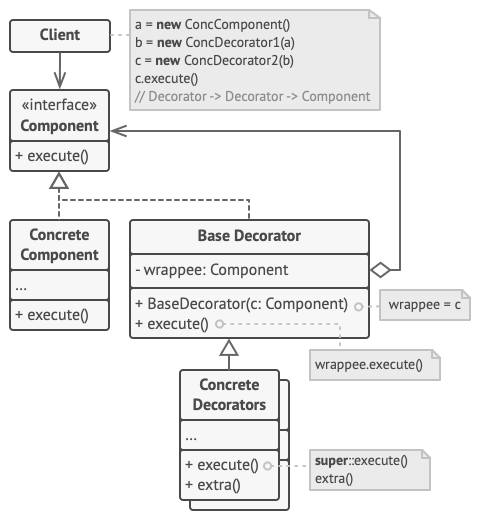
\includegraphics[width=0.5\textwidth]{img/DecoratorDesignPattern.png}
	\caption{Decorator design pattern}
	Source: \autocite{img:Decorator}
	\label{fig:decorator}
\end{figure}

The Extension Objects design pattern (as shown in \cref{fig:extension objects}) could
also be used to structure the game engine. The Extension Objects design pattern
allows to modify an object's propperties/behavior by adding one (or more) Extensions.
The object that is modified, could be the gameObject and the components could be the
Extensions. This is quite the same as the required API. An advantage is, that the
client (which is the scene in our case) can call all kind of different Extension's
methods (depending on the kind of Externsion, e.g.~the method \codeinline{render()}
for the sprite Extension and the method \codeinline{update()} for the script
Extension). In other words, the interfaces of the different Extensions should not be
the same. This is way more flexible than the Decorator design pattern. A disadvantage
is that the data and functionality are in the same class (namely inside the Extion's
methods), so it's not sepperated. Another disadvantage is that the Extension Objects
design pattern can be quite slow, because objects are scattered in memory (and it is
very hard to quickly get their memory address)
\autocite{man:ExtensionObjectDesignPattern, man:extionsionObjectsStackOverflow}.

\begin{figure}
	\centering
	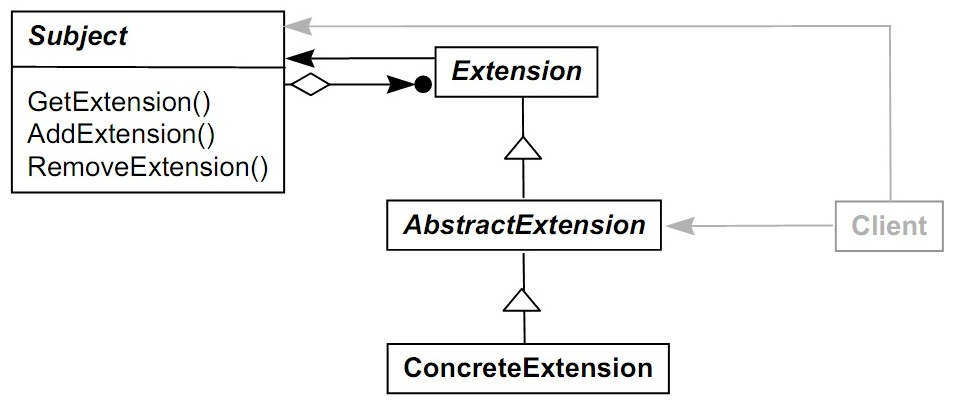
\includegraphics[width=0.5\textwidth]{img/ExtensionObjects.jpg}
	\caption{Extension Objects design pattern}
	Source: \autocite{img:extionsionObjects}
	\label{fig:extension objects}
\end{figure}

Another (very popular) design pattern to structure the game engine, is the Entity
Component System (\gls{ecs}) (as shown in \cref{fig:ECS Block Diagram}). The
\gls{ecs} is made out of three main subsystems, namely entities, components and
systems. Entities are just IDs. An entity is made out of a gameObject and one (or
more) components. Components are the classes that hold the data. The components
determine what kind of entity it is (e.g.~a sprite, audio, and so on). Systems take
care of the behavior of the entities. Systems mainly read and write the enity's
components data. The \gls{ecs} clearly distinguishes the data (components) from the
functionality (systems), which is an advantage.

\begin{figure}
	\centering
	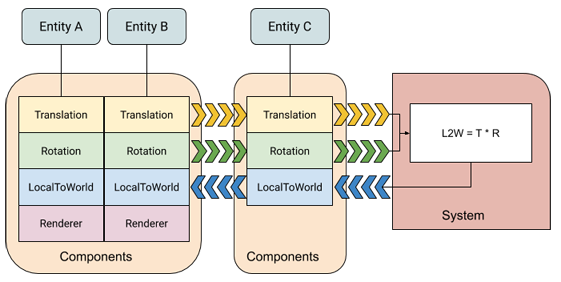
\includegraphics[width=0.5\textwidth]{img/ECSBlockDiagram.png}
	\caption{ECS design pattern}
	Source: \autocite{img:ECSBlockDiagram}
	\label{fig:ECS Block Diagram}
\end{figure}

The \gls{ecs} is normally equipped with a component manager (as shown in
\cref{fig:ECS Component manager}). The component manager keeps track of the entities
(Alien, Player, Target, etc in \cref{fig:ECS Component manager}) and the connected
components (Position, Movement, Render, etc in \cref{fig:ECS Component manager}). The
component manager stores two lists (key value pairs). The key of the first list is
the ID of an entity, and the value of this list are the connected components. The key
of the second list is the component, and the value of this list are the entities that
have this component. These two lists make it possible to very quickly gather
components or entities. This makes the \gls{ecs} very fast, which is of course an
advantage \autocite{man:ECSComponentManager}.

\begin{figure}
	\centering
	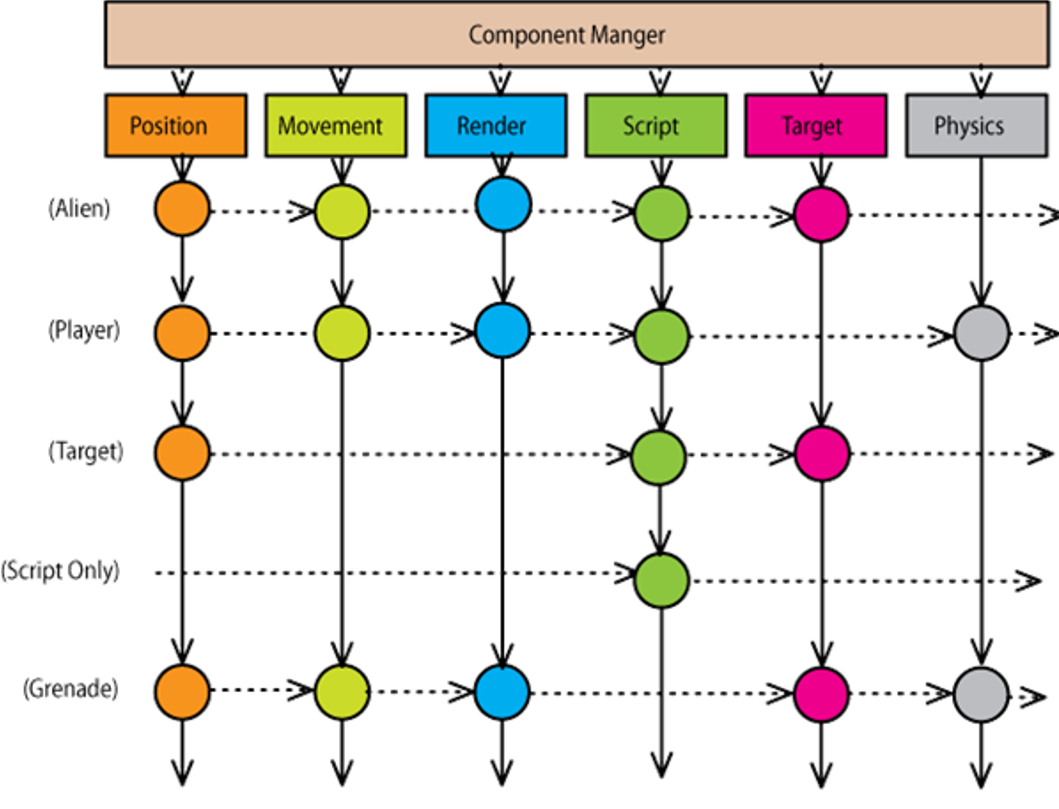
\includegraphics[width=0.5\textwidth]{img/ECSComponentManager.png}
	\caption{ECS Component manager}
	Source: \autocite{img:ECSComponentSystem}
	\label{fig:ECS Component manager}
\end{figure}

Another aspect that makes the \gls{ecs} very fast, is that a system can handle all
components (of the same type) together at once. This is possible because all entities
are independent of each other.

There are many ways of implementing the systems. Some say that each component type
has their own system. This interpretation of the systems does not take the interplay
of different component types, into account. A less restrictive approach is to let
different systems deal with all components they should be concerned with. For
instance a Physics Systems should be aware of Collision Components and Rigidbody
Components, as both probably contain necessary information regarding physics
simulation. It's best to see systems as ``closed environments''. That is, they do not
take ownership of entities nor components. They do access them through independent
manager objects, which in turn will take care of the entities and components
life-cycle \autocite{man:ECSExplanation}.

Sometimes systems, entities and even components need to cummincate with each other.
This might be very hard because systems, entities and components are more or less
independent. One option is to use an event systems. A system, entity and component
can raise an event and other systems, entities and components can react to that
event. This is what makes the \gls{ecs} a complicated system (disadvantage)
\autocite{man:ECSExplanation}.

There are many C/C++ libraries available, completely dedicated to \gls{ecs}. The most
popular libraries are shown in \cref{tab:popularECSLibraries}. The popularity is
based on the amount of stars on GitHub.

\begin{table}
	\centering
	\begin{tabular}{ll@{\qquad}lr}
		\toprule
		\textbf{Name} & \textbf{Short Description} & \textbf{Stars} & \textbf{License}\\
		\midrule
		EnTT & Fast and reliable entity-component system & 10k & MIT\\
		Flecs & A Multithreaded Entity Component System & 6.3k & MIT\\
		EntityX & Fast, type-safe C++ entity component system & 2.2k & MIT\\
		\bottomrule
	\end{tabular}
	\caption{Popular \gls{ecs} libraries}
	Source: \autocite{github:awesome-ecs}
	\label{tab:popularECSLibraries}
\end{table}

TODO: Add library benchmark to find the best library.

It is, of course, not necessary to use a library to implement an \gls{ecs}
architecture. However, it seems very hard to achieve the same performance as a
library \autocite{github:ecsfaq}.

\subsection{Conclusion}

\section{Gameobjects/components}
\label{sec:Gameobjects/components}

\subsection{Introduction}

One of the requirements of our customer, is that the game engine's structure is
similar to Unity. The customer has created a class diagram of the game engine's API,
which is (of course) very similar to Unity. One of the most important parts of the
class diagram is a so-called gameObject (with several components). It's needed to
understand the exact meaning/function of these gameObjects, that's why this research
question arose.

\subsection{Findings}

A gameObject is the most important concept in Unity. Every object in a game is a
GameObject, from characters and collectible items to the lights, cameras and special
effects. However, a gameObject itself can't do anything on its own. A gameObject
needs to be given properties before it can become a character, an envirnment, or a
special effect. \autocite{man:unityGameobjects}

A gameObject can be seen as a container for components. Components are the properties
of the gameObject. A few examples of components are sprites, animators, audioSources,
and so on. Multiple (different) components can be assigned to a single gameObject
(e.g.~a sprite and an audioSource).

Since we now know that a gameObject needs components to do something, it's obvious
that there should be a way to add components to a gameObject. Some components
(e.g.~the behaviorScript component) should also be able to reference to its
gameObject.

Each gameObject always has one transform class. The transform class describes the
position, rotation, and scale within the scene. Some component use this information
to e.g.~scale a sprite. Other components eddit this information to e.g.~model
gravity. \autocite{man:unityTransformClass}

A gameObject can have one (or multiple) children gameObject(s). All children
gameObjects, of course, also have one transform class. However, the position,
rotation, and scale of this class, is always the same as the child's parent. A child
can not have more than one parent. \autocite{man:unityTransformClass}

\subsection{Conclusion}

\section{Third-party Tools}

\subsection{Introduction}

Developing a game engine from scratch requires a significant amount of time, as many
different features are necessary. Fortunately, some of these features have already
been developed and can be reused in the form of frameworks and third-party
tools/libraries. The decision to use third-party libraries, and the selection of
which ones to use, directly influences the development process of the game engine. In
this section, several third-party frameworks and tools available for use are
described.

\subsection{Findings}

\subsubsection{Media Frameworks}

A game engine must have the ability to handle user input, render graphics, and
process audio. Several large frameworks are available that provide these features and
are already widely used by other game engines. The two most popular and
best-supported options are \gls{sdl2} and \gls{sfml}.

\paragraph{SDL2}

% TODO: ref?sdl2
According to its official website, \gls{sdl2} is \emph{``a cross-platform development
library designed to provide low-level access to audio, keyboard, mouse, joystick, and
graphics hardware via \gls{opengl} and \gls{d3d}. It is used by video playback
software, emulators, and popular games, including Valve's award-winning catalog and
many Humble Bundle games.''} \gls{sdl2} is written in the C programming language, and
therefore, structs and functions are used instead of objects and methods.

\begin{comparison}
	\pro{Controller support is provided.}
	\pro{2D and 3D rendering are supported.}
	\pro{Broad multiplatform support is offered, including older consoles such as the
	Wii.}
	\pro{Low-level control is available.}
	\pro{A large community ensures wide usage.}
	\pro{Extended libraries can be used to add functionalities, such as SDL\_Mixer for
	sound.}
	\con{A limited built-in 2D renderer is provided.}
	\con{Extended libraries require setup.}
\end{comparison}

\paragraph{SFML}

\gls{sfml} is a simple framework consisting of five modules: audio, graphics,
network, system, and window. This framework, written in C++, was designed to simplify
game development.

\begin{comparison}
	\pro{Object-oriented design is provided since it is written in C++.}
	\pro{A built-in 2D renderer is available for ease of use.}
	\pro{A built-in audio system is included.}
	\pro{Cross-platform support is available for Linux, Windows, and macOS.}
	\pro{Networking capabilities are provided for multiplayer or networked
	applications.}
	\con{The 2D rendering engine may experience performance issues in large-scale
	games.}
	\con{The community is smaller compared to \gls{sdl2}.}
	\con{No native 3D support is provided.}
	\con{Not all image formats are supported.}
\end{comparison}

\subsubsection{Audio}

for audio some options could be: FMOD, Wwise, or iirKlang

\subsection{Conclusion}

\section{Resource manager}

\subsection{Introduction}

\subsection{Findings}

\subsection{unity formats}
Unity has many different asset file types that can be imported to use for a game \href{https://docs.unity3d.com/Manual/BuiltInImporters.html}{unity imports}. The most important formats are the audio, text and sprite formats.

\paragraph{Audio}

The unity engine supports a lot of different audio formats:
\begin{itemize}
	\item ogg.
	\item aif.
	\item aiff.
	\item flac.
	\item wav.
	\item mp3.
	\item mod.
	\item it.
	\item s3m.
	\item xm.
\end{itemize}

\paragraph{Sprite formats}

Unity supports many different image formats:
\begin{itemize}
	\item jpg.
	\item jpeg.
	\item tif/tiff.
	\item tga.
	\item gif.
	\item png.
	\item psd.
	\item bmp.
	\item iff.
	\item pict.
	\item pic.
	\item pct.
	\item exr.
	\item hdr.
\end{itemize}

\subsection{Audio Format} The choice of audio format for the Crepe game engine depends on several factors, including sound quality, memory usage, and licensing. According to various sources \href{https://dev.to/tenry/comparison-of-audio-formats-for-games-jak}{comparison audio formats}, \href{https://www.universityofgames.net/articles/audio-file-formats-used-in-game-development/}{Audio files in games} , the most commonly used audio formats in game development are WAV, MP3, and Ogg.

\paragraph{Licensing} Historically, MP3 had patents on the audio format, but these restrictions have expired. Ogg and FLAC, both developed by Xiph.Org, are open-source formats. Additionally, the WAV format, though widely used, does not require a specific license for distribution.

\paragraph{Conclusion} For the Crepe game engine, Ogg and FLAC are the preferred audio formats due to their open-source licenses and high compatibility. FLAC is ideal for high-quality audio with minimal compression, while Ogg is better suited for lower-quality audio that requires reduced memory usage. Both formats come from the same non-profit organization, Xiph.Org, ensuring that they align with open-source values and licensing flexibility.


\subsection{Conclusion}

\section{Rendering}

\subsection{Introduction}

\subsection{Findings}

\subsection{Conclusion}

\section{Event manager/game loop}

\subsection{Introduction}

\subsection{Findings}

\subsection{Conclusion}

% TODO: this entire section
\section{Profiling and debugging}

% Which profiling and debugging features are wanted?
% How to provide those profiling and debugging features?
% Can most of the profiling/debugging be handled by external tools?

% Ideas:
% - flame graph
% - watchtable (combine w/ fps/speed control overlay?)
% - debug printing utility functions

\subsection{Introduction}

\subsection{Findings}

\subsubsection{Callgrind}

\begin{comparison}
	\pro{Source code does not need to be modified for profiling}
	\con{Execution speed is severely impacted}
\end{comparison}

\subsection{Conclusion}

\section{Audio}

The game engine is required to have an audio system
\autocite[\ref{req:audio}]{crepe:requirements}. Since writing a custom real-time
audio mixing engine is outside the scope of this project\mref, this section compares
various standalone audio libraries for suitability in the engine.

\subsection{Libraries}
\label{sec:audio:libs}

After searching for libraries (search terms: `dynamic/adaptive audio', `real-time
audio', `audio library', `game audio engine'), several libraries were found. These
libraries were checked against the audio engine requirements
\autocite{crepe:requirements} and then tested by writing the same benchmark-style
\gls{poc} using the remaining qualifying libraries:\noparbreak
\begin{enumerate}
	\item Load a background track (Ogg Vorbis)
	\item Load three short samples (WAV)
	\item Start the background track
	\item Play each sample sequentially while pausing and resuming the background track
	\item Play all samples simultaniously
	\item Stop all audio and exit
\end{enumerate}

Of these libraries the following were determined to be unsuitable for use in this
project due to various reasons:\noparbreak
\begin{description}
	\item[FMOD \autocite{lib:fmod}] Is proprietary (violates \cref{req:lib:license})
	\item[PortAudio \autocite{lib:portaudio}] Does not handle mixing
	\item[miniaudio \autocite{lib:miniaudio}] With finished \gls{poc}, but dropped due
		to very limited codec support (WAV, MP3 and FLAC only); Also does not have an
		\gls{api} reference (only programming manual)
	\item[YSE \autocite{lib:yse}] Attempted to write \gls{poc}, but CMake configuration
		in repository is broken; This project seems to have been abandoned
\end{description}

The only library that remained after these tests is SoLoud \autocite{lib:soloud}. It
is Zlib/LibPng licensed and provides a high-level object-oriented C++ \gls{api}.

\subsection{Conclusion}
\label{sec:audio:conclusion}

Due to a severe shortage of libraries that fit our requirements, SoLoud appears to be
the most suitable (and only) audio library for use in this project.

\section{Physics}

\subsection{Introduction}

\subsection{Findings}

\subsection{Conclusion}

\section{Scripting}

\subsection{Introduction}

\subsection{Findings}

\subsection{Conclusion}

\section{Audio}

\subsection{Introduction}

\subsection{Findings}

\subsection{Conclusion}

\section{AI}

\subsection{Introduction}

\subsection{Findings}

\subsection{Conclusion}

\end{document}
